\documentclass{scrartcl}
% Packages
\usepackage{hyperref}
\usepackage{tikz}
\usepackage{amsmath}
\usepackage{pifont}
\usepackage{mathrsfs}
\usetikzlibrary{arrows.meta, positioning}

\definecolor{darkgreen}{rgb}{0.0, 0.5, 0.0}


\title{Summer 2024 Report}
\author{Sam Arkle}
\date{\today}

\begin{document}

\maketitle

\section{Introduction}
This is a report on the progress I have made during the summer of 2024 working with Dr. Polonsky \footnote{Assisstant Professor, Department of Computer Science, Appalachian State University.}. I have been writing on the topic of relations, working primarily from Term Rewriting Systems (TeReSe) \footnote{(Term Rewriting Systems. (2003). United Kingdom: Cambridge University Press.)}.
The objective of this work has been to both develop a formal understanding of relations and to build a library in Agda \footnote{\href{https://github.com/DrPolonsky/LAM/tree/main/Relations}{Github repository for this project's code}} that will be used as a foundation to further work in theoretical computer science.
\\
I have been focussed on Chapter 1 of TeReSe which covers abstract reduction systems (ARS) as well as the appendix (sections 1-3) which provides the necessary mathematical background for the rest of the book (e.g. relations, ordinals, inductive definitions and the Knaster-Tarski lemma). Where the book has made use of classical logic I have investigated the possibility of using constructive alternatives.

\section{Relations}

\subsection{Well-foundedness}
\textcolor{red}{Talk about the different types of wellfoundedness, starting with the one given in the book, the reason for thinking it is classical and not constructive, and provide an image showing the relation between the notions of wellfoundedness we have. Talk about future work in this area.}
\\
We have worked with four different notions of well-foundedness in order to explore the connections between them. These four notions each depend on one of the following four definitions:
\begin{enumerate}
    \item accessible \textcolor{red}{For these definitinos is it best to just use the code from agda which is clear, or should we be trying to provide a more 'human' definition to accompany the code?}
    \item inductive predicate
    \item minimal element
    \item non-decreasing index
\end{enumerate}
The four main notions of a relation \textit{R} being well-founded a set \textit{S} we have worked with are:
\begin{enumerate}
    \item \textit{R} is well-founded if every element is \textit{R}-accessible (where an element \textit{x} is \textit{R}-accessible if all elements \textit{R}-below \textit{x}  are themselves \textit{R}-accessible).
    \item \textit{R} is well-founded if every inductive predicate is universally true (where a predicate $\varphi$ is inductive if $\varphi\,x$ is true whenever $\varphi\,y$ is true for all elements $y$ $R$-below $x$).
    \item \textit{R} is well-founded if every non-empty subset of $S$ has a minimal element with respect to $R$.
    \item \textit{R} is well-founded if every sequence contains a non-decreasing index.
\end{enumerate}
Further, we explored weaker variants of these notions of well-foundedness by defining well-foundedness using double negation:
\begin{enumerate}
    \item \textit{R} is well-founded if every element is $\lnot \lnot$  \textit{R}-accessible.
    \item \textit{R} is well-founded if for every inductive predicate $\varphi \; \lnot \lnot \varphi \; x$.
    \item \textit{R} is well-founded if for every non-empty subset of $S$ there is $\lnot \lnot$ a minimal element with respect to $R$.
    \item \textit{R} is well-founded if there is no infinite $R$-decreasing sequence in $S$ (this is the definition of well-foundedness found in TeReSe).
\end{enumerate}

The following graphic illustrates the connections we have found between these definitions and those we are still seeking to find. Green arrows indicate that a definition can be translated into another, red arrows indicate that we believe a translation should be possible but we have not yet found it.

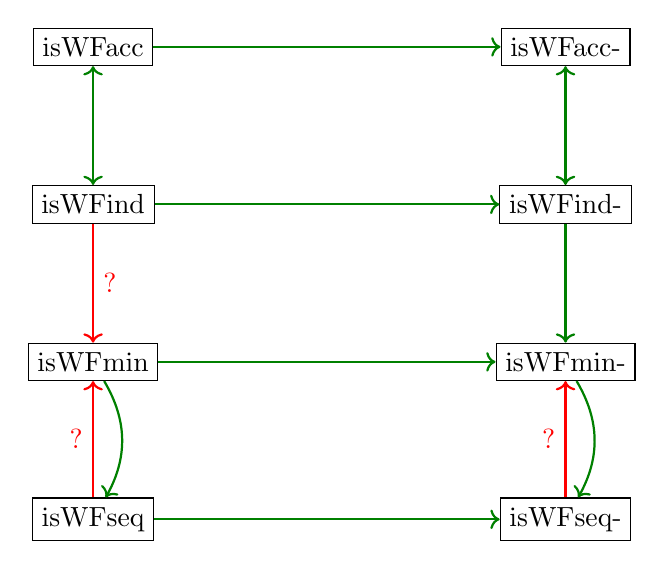
\begin{tikzpicture}[node distance=2cm, auto]
    % Standard definitions
    \node (std1) [draw] {isWFacc};
    \node (std2) [below of=std1, draw] {isWFind};
    \node (std3) [below of=std2, draw] {isWFmin};
    \node (std4) [below of=std3, draw] {isWFseq};

    % Weaker definitions
    \node (weak1) [right of=std1, xshift=4cm, draw] {isWFacc-};
    \node (weak2) [below of=weak1, draw] {isWFind-};
    \node (weak3) [below of=weak2, draw] {isWFmin-};
    \node (weak4) [below of=weak3, draw] {isWFseq-};

    % Arrows
    \draw[->, thick, darkgreen] (std1) -- (weak1);
    \draw[<->, thick, darkgreen] (std1) -- (std2);
    \draw[<->, thick, darkgreen] (weak1) -- (weak2);
    \draw[->, thick, darkgreen] (std2) -- (weak2);
    \draw[->, thick, red] (std2) -- (std3) node[pos=0.5, right, red] {?};
    \draw[->, thick, darkgreen] (weak2) -- (weak3);
    \draw[->, thick, darkgreen] (std3) -- (weak3);
    \draw[->, thick, darkgreen, bend left] (std3) to (std4);
    \draw[->, thick, darkgreen, bend left] (weak3) to (weak4);
    \draw[->, thick, darkgreen] (std4) to (weak4);
    \draw[->, thick, red, bend left] (std4) -- (std3) node[pos=0.5, left, red] {?};
    \draw[->, thick, red, bend left] (weak4) -- (weak3) node[pos=0.5, left, red] {?};
\end{tikzpicture}

As future work we want to know whether the missing reductions can be defined, or what the minimal additional requirements are for making those reductions.

\subsection{Definitions}
\textcolor{red}{Go through some of the main definitions formalised from Terese, focussing on where we have used constructive alternatives to the classically given definitions
Could talk here about omega bounded stuff too!}
\\
One aspect of the project has been working through the definitions, propositions, and theorems in TeReSe and formalising them in Agda.
For example, in TeReSe the diamond property is defined:
\begin{center}
    $a \in A$ has the \textit{diamond property} if $\forall b, c \in A (c \leftarrow a \rightarrow b \implies \exists d \in A c \rightarrow d \leftarrow b)$. The reduction relation $\rightarrow$ has the \textit{diamond property} if every $a \in A$ has the \textit{diamond property}.
\end{center}
In Agda we have defined the diamond property as:
\begin{flushleft}
    \texttt{\ding{117} : Set}\\
    \texttt{\ding{117} = $\forall a, b, c \rightarrow R_{\alpha} a b \rightarrow R_{\alpha} a c \rightarrow \Sigma[ d \in A ] (R_{\alpha} b d \times R_{\alpha} c d)$}
\end{flushleft}
In formalising the propostions and theorems we also provided solutions to them. \\
The remainder of this section highlights definitions or proofs we hae expressed differently to TeReSe along with an explanation of why we have done so.

\subsubsection{Strongly Normalizing}
\begin{center}
    In TeReSe: $a \in A$ is \textit{strongly normalizing} if every reduction sequence starting from $a$ is finite. The reduciton relation $\rightarrow$ is \textit{strongly normalizing} (SN) if every $a \in A$ is strongly normalizing.
\end{center}
In Agda we have defined strongly normalizing as:

\begin{flushleft}
    \texttt{data is\_-accessible\_ : $\mathscr{P} A$ where}\\
    \texttt{\ \ \ \ acc : $\forall$ \{x : A\} $\rightarrow$ ($\forall$ y $\rightarrow$ R y x $\rightarrow$ is\_-accessible\_ y) $\rightarrow$ \quad is\_-accessible\_ x}\\
    \texttt{is\_SNacc\_ : $\mathscr{P} A$}\\
    \texttt{is\_SNacc\_ x = is (\textasciitilde R R) -accessible x}\\
    \texttt{is\_SN\_ : $\mathscr{P} A$}\\
    \texttt{is\_SN\_ = is\_SNacc\_}
\end{flushleft}


\subsection{Knaster Tarski}
Go through different proofs Here

\subsection{Newmans lemma}
What it is and the different definitions again

\subsection{}

\section{Notes from 08.29}

\begin{enumerate}
  \item Try to ``fix'' CP by changing $R$ into $R^r$
  \item Finish formulating the ``compactness property".  Two candidates:
  \begin{itemize}
    \item ``Every cocone for a given infinite sequence loops back to some point in the sequence"
    \item ``If an $R^*$-sequence has a cocone then it's constant after some point on.''
  \end{itemize}
  \item Add the definition of "recurrent element"
\end{enumerate}
\end{document}
